\section{Odbiornik}

Centralną część prezentowanego prototypu stanowi odbiornik.
Jego zadaniem jest wysyłanie sygnałów sterujących do nadajnika, zbieranie ultradźwięków z otoczenia oraz przesyłanie 
ich do komputera w celu dalszej analizy.
Odbiornik składa się z następujący części (rysunek \ref{fig:odbiornik_szkic}):

\begin{itemize}
 \item trzech modułów ultradźwiękowych przetwarzających dźwięk na sygnał elektryczny,
 \item płytki prototypowej \textit{stm32f4-discovery} \cite{bib:stm32f4Discovery} odpowiadającej za komunikację z komputerem,
 \item przystawki do \textit{stm32f4-discovery} przystosowującej sygnały elektryczne z modułów ultradźwiękowych
  do poziomów akceptowalnych przez tę płytkę oraz wyprowadzającej sygnały sterujące nadajnikiem,
 \item ramy, na której umieszczono moduły ultradźwiękowe.
\end{itemize}


\rysunek{odbiornik_szkic}{Szkic odbiornika}{\label{fig:odbiornik_szkic}}


\section{Budowa i zasada działania odbiornika}

Głównym elementem odbiornika jest płytka prototypowa \textit{stm32f4-discovery} \cite{bib:stm32f4Discovery}.
 Umożliwia ona komunikację wszystkich komponentów z komputerem.
\textit{Stm32f4-discovery} wyposażona jest w procesor STM32F407VGT6 \cite{bib:stm32f407} (oparty o rdzeń ARM Cortex M4), 
który zawiera trzy 12-bitowe przetworniki
analogowo-cyfrowe umożliwiające próbkowanie z prędkością do \SI{2,4}{MSPS} 
(ang. \textit{MSPS -- Mega-Samples Per Second} -- milion próbek na sekundę). Przetworniki te wykorzystane zostały do próbkowania
sygnałów pochodzących z modułów ultradźwiękowych. Płytka umożliwia również komunikację z komputerem przez 
port USB z prędkością \SI{12}{MB/s}. Znajduje się na niej także programator
umożliwiający programowanie procesora za pośrednictwem dodatkowego portu USB.

Na potrzeby odbiornika powstało dedykowane oprogramowanie w C sterujące procesorem.
Zostało ono oparte na bibliotece \textit{stm32 usb 101} \cite{bib:stm32_usb_101} zapewniającej komunikację z komputerem. 
Do biblioteki dodano obsługę przetworników analogowo-cyfrowych oraz możliwość sterowania nadajnikiem.
Program przez port USB dostaje instrukcję, który z czterech głośników ma nadawać, i przekazuje ją
dalej do nadajnika wraz z sygnałem wyzwalającym. Następnie uruchamiane są równocześnie trzy przetworniki analogowo-cyfrowe, które 
próbkują odbierany dźwięk i poprzez DMA zapisują wynik w pamięci procesora.
Częstotliwość pracy przetworników ustawiono na \SI{1,6}{MSPS}, co daje 40 próbek na jeden okres sygnału o częstotliwości \SI{40}{kHz}.
Po zebraniu w sumie $3\times\SI{16}{k}=\SI{48}{k}$ próbek całość przesyłana jest do komputera w celu dalszej analizy.
Proces powtarza się dla każdego z czterech głośników nadajnika, 
co w sumie daje 12 sygnałów, na podstawie których wyznaczona zostaje 
pozycja w przestrzeni oraz orientacja nadajnika.

Całą elektronikę osadzono na ramie w kształcie trójkąta zbudowanej z rur PCV  (rysunek \ref{fig:trojkat}). 
Odległości pomiędzy modułami ultradźwiękowymi są z góry ustalone, co ułatwia dalsze obliczenia.

Warto zaznaczyć, że dla dźwięku poruszającego się z prędkością \SI{340}{m/s} długość wykorzystanej 
fali dźwiękowej wynosi \SI{8.5}{mm}, co przy 
pomiarze 40 próbek na jeden okres daje rozdzielczość pomiaru odległości mniejszą niż \SI{0.5}{mm} (dokładnie \SI{0.2125}{mm}).
Błąd pomiaru trudno jednak oszacować, ponieważ  zależy on od aktualnej prędkości
dźwięku, a ta zmienia się w czasie wraz ze zmianą warunków atmosferycznych.

 \begin{figure}[h]
    \centering
    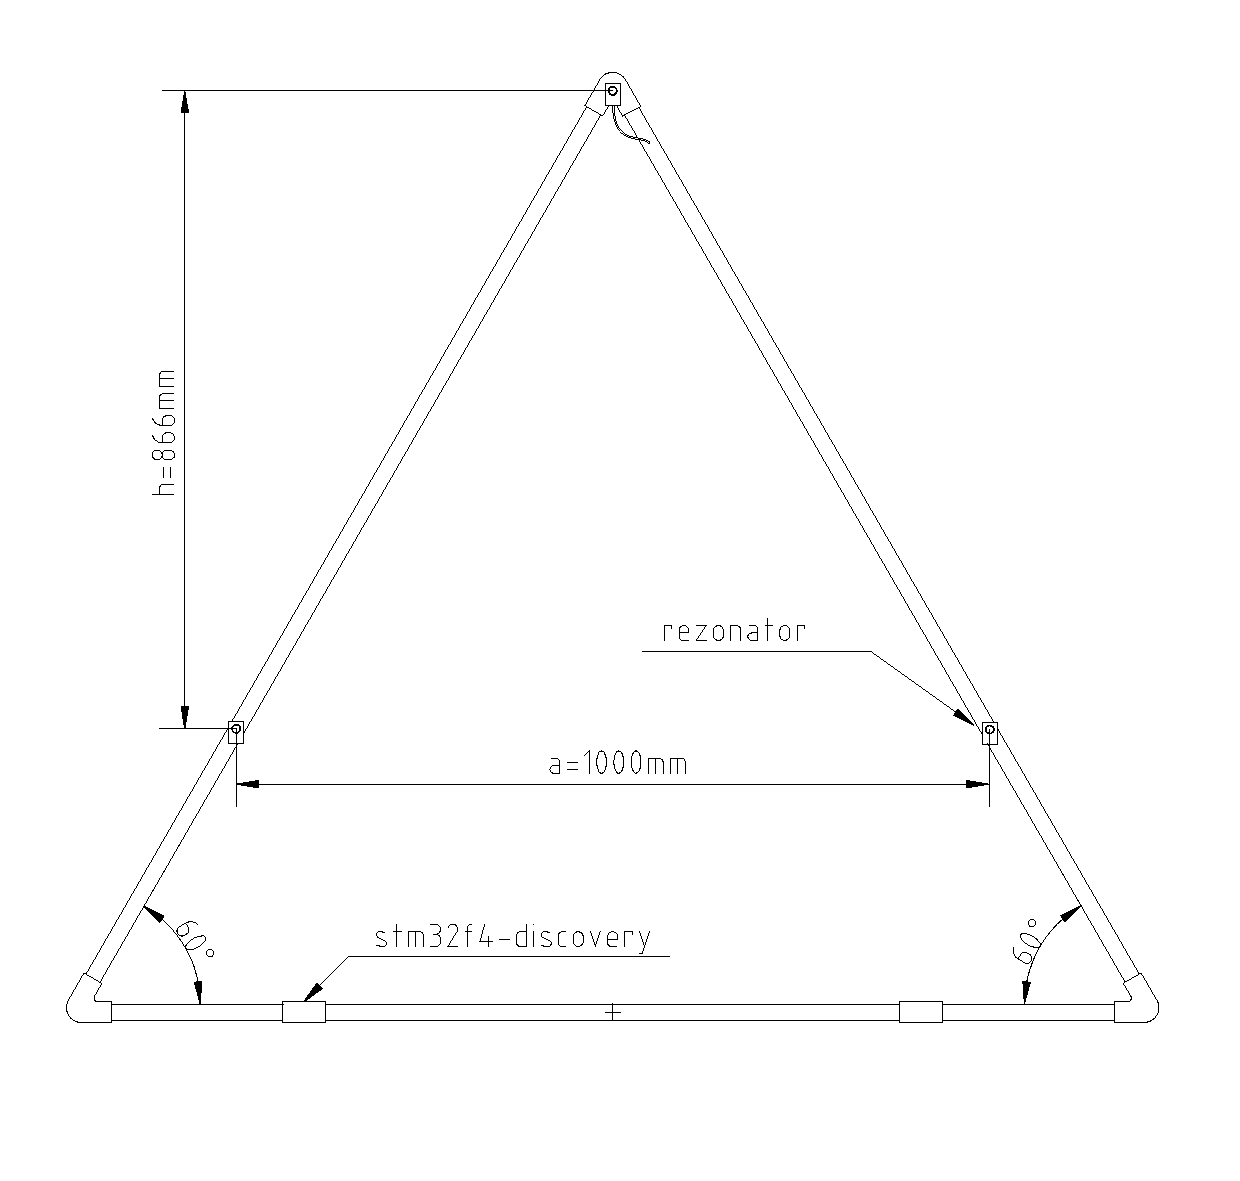
\includegraphics[width=0.8\textwidth, trim= 0mm 20mm 0mm 0mm,clip]{trojkat}
    \caption{Szkic ramy odbiornika}
    \label{fig:trojkat}
\end{figure}


\section{Budowa modułu ultradźwiękowego}

Odbiornik wyposażono w trzy moduły ultradźwiękowe, których zadaniem jest 
zbieranie ultradźwięków z trzech różnych  punktów.
Każdy moduł zawiera przetwornik piezoelektryczny (mikrofon) 40SR-12 \cite{bib:40ST12},
który przetwarza sygnał akustyczny na odpowiadający mu sygnał elektryczny, oraz wzmacniacze operacyjne 
wstępnie zwiększające amplitudę sygnału, który przesyłany jest dalej do przystawki.
Rysunek \ref{fig:odbiornik_ultra} przedstawia schemat modułu ultradźwiękowego.

\rysunek{receiver}{Schemat modułu ultradźwiękowego}{\label{fig:odbiornik_ultra}}

Wzmacniacz operacyjny IC1A wraz z kondensatorem C2 i rezystorem R1 pracuje 
jako przedwzmacniacz ładunkowy \cite{bib:wzm_ladunkowy}.
Ładunek wytworzony na przetworniku piezoelektrycznym SP1 zostaje w całości przeniesiony na kondensator C2 
(wzmacniacz utrzymuje różnicę potencjałów między dodatnim a ujemnym wejściem na zerowym poziomie).
W rezultacie na kondensatorze C2 pojawia się napięcie proporcjonalne do wartości odebranego sygnału.
Do rozładowania kondensatora C2 służy rezystor R1.
R1 i C2 działają również jako filtr dolnoprzepustowy.

Wzmacniacz IC1B z rezystorami R5 i R4 oraz kondensatorami C3, C7 i C8 pracuje jako wzmacniacz napięciowy wzbogacony o 
filtr pasmowoprzepustowy.
Sygnał z IC1B za pośrednictwem wtyczki JP1 dociera do przystawki współpracującej z \textit{stm32f4-discovery}.

W celu zminimalizowania zakłóceń zastosowano niskoszumowe wzmacniacze operacyjne
mieszczące się w jednym układzie scalonym NE5532 \cite{bib:ne5532}. 
Dodatkowo płytka drukowana jest ekranowana.


\section{Przystawka do \textit{stm32f4-discovery}}

Sygnał z modułów ultradźwiękowych dociera do \textit{stm32f4-discovery} za pośrednictwem specjalnej przystawki.
Schemat budowy przystawki przedstawia rysunek \ref{fig:przystawka}.
Przystawka przystosowuje maksymalne amplitudy zebranych sygnałów do wartości akceptowalnych przez  
przetworniki analogowo-cyfrowe procesora STM32F407VGT6.
Wartości te muszą mieścić się w zakresie od \SI{0}{V} do \SI{3,3}{V}.

Zastosowano w niej układ TLV2774 \cite{bib:TLV2774}, który zawiera 4 wzmacniacze operacyjne typu
\textit{rail-to-rail}. Trzy z nich wykorzystano jako ostatni stopień wzmocnienia sygnałów ultradźwiękowych. 
Wzmacniacze operacyjne pracują w układzie odwracającym, którego wzmocnienie można regulować odpowiednio potencjometrami R8, R9 oraz R10. 
Podłączono je do wspólnego, również regulowanego (przy użyciu potencjometru R7) napięcia odniesienia.
Przystawka zawiera także stabilizator napięcia LM78M05CDT \cite{bib:LM78M05CDT}, który po podłączeniu 
do JP4 baterii \SI{12}{V} dostarcza zasilanie do wszystkich komponentów. 
Istnieje możliwość odcięcia zasilania przez rozwarcie JP5, co jest konieczne podczas programowania
STM32F407VGT6, by zapobiec uszkodzeniu stabilizatora napięcia.
Z przystawki przez wtyczkę JP6 wyprowadzono również sygnały sterujące nadajnikiem oraz zasilanie.
Wtyczka JP6 połączona jest z wtyczką SV1 nadajnika (rysunek \ref{fig:nadajnik_schemat}) sześciometrowym kablem.

 \begin{figure}[h]
    \centering
    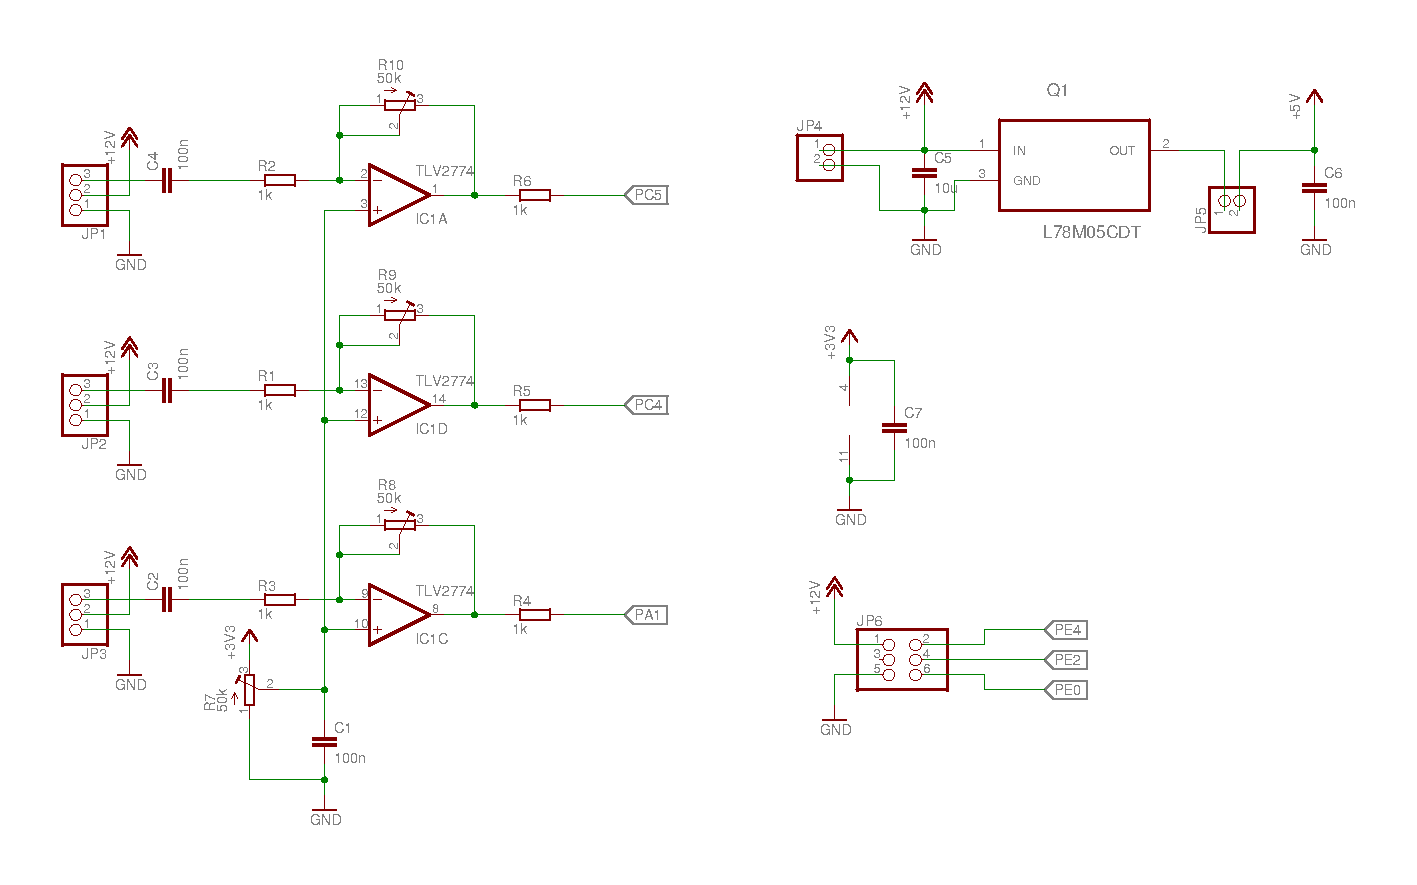
\includegraphics[width=1\textwidth, trim= 5mm 0mm 0mm 0mm,clip]{mainboard2}
    \caption{Schemat budowy przystawki do \textit{stm32f4-discovery}}
    \label{fig:przystawka}
\end{figure}


